\documentclass[10pt,a4paper,twoside]{article}

\usepackage[T1]{fontenc}
\usepackage[latin1,utf8]{inputenc}

\usepackage{lmodern}

\usepackage[pdftex]{graphicx} 

\usepackage[tracking=true]{microtype}
               
                               
\usepackage{amsmath,amssymb,amsthm}
\usepackage{xfrac}
\usepackage{mathrsfs}
\usepackage{mathtools}
\usepackage{grffile}  

\usepackage{bbm} %for use of identity-matrix
\usepackage{dsfont}

\usepackage[]{subfigure}

\usepackage{verbatim}

\usepackage{color}
\usepackage{hyperref}

\usepackage{accents}
\usepackage{textcomp}
\usepackage{multirow}
\usepackage{booktabs}
\usepackage{float}

\usepackage[numberedbib]{apacite}
\bibliographystyle{apacite}
\usepackage[flushleft]{threeparttable}
\usepackage{tabulary}
\usepackage{indentfirst}

\setlength{\columnsep}{20pt}

\usepackage{geometry}
\geometry{a4paper,left=30mm,right=25mm, top=20mm, bottom=25mm}

\usepackage{fancyhdr}
\pagestyle{fancy}
\fancyhf{}
\rhead{André Crescenzo}
\lhead{Computer-aided Design of Bio-inspired Nanoporous Silica Materials}
\lfoot{\today}
\rfoot{\thepage}

\usepackage{abstract}
\usepackage{authblk}

\title{A Coarse-grain model for Bolaamphiphiles in presence  of Silica}
\author[1,2]{André Crescenzo\thanks{ Corresponding author.\\ Email: \ \texttt{andre.crescenzo.2014@uni.strath.ac.uk}}}
\author[1]{Alessia Centi\thanks{ Email: \ \texttt{alessia.centi@strath.ac.uk}}}
\author[1]{Miguel Jorge\thanks{Email: \ \texttt{miguel.jorge@strath.ac.uk}}}
\affil[1]{Department of Chemical and Process Engineering, University of Strathclyde}
\affil[2]{Departamento de Engenharia Química da Escola Politécnica, Universidade de São Paulo}
\renewcommand\Authands{ and }
\date{\today \\
\begin{abstract}
\textbf{Aim:} Finish my job!\\
\textbf{Conclusion:}Repeating the results is not drawing a conclusion.
\begin{tabular}
& \textbf{Keywords}: Latex$\cdot$ Bibtex  $\cdot$ Scientific Paper $\cdot$ More Scientific Papers $\cdot$ More Scientific Papers  $\cdot$ More Scientific Papers $\cdot$ More Scientific Papers $\cdot$ More Scientific Papers $\cdot$ More Scientific Papers 
\end{tabular}
\end{abstract}}

\pagenumbering{roman}

\begin{document}

\begin{titlepage}

\newcommand{\HRule}{\rule{\linewidth}{0.5mm}} 

\center 
 
\begin{figure*}[ht!]
	
\includegraphics[width=1 \textwidth]{./images/StrathLogo}
\end{figure*}


\textsc{\LARGE University of Strathclyde}\\[1.5cm] 
\textsc{\Large Department of Chemical \& Process Engineering}\\[0.5cm] 
\textsc{\large M.Eng Chemical \& Process Engineering 18530}\\[0.5cm] 


\HRule \\[0.4cm]
{ \huge \bfseries Computer-aided Design of Bio-inspired Nanoporous Silica Materials}\\[0.4cm] % Title of your document
\HRule \\[1.5cm]
 

\begin{minipage}{0.4\textwidth}
\begin{flushleft} \large
\emph{Author:}\\
André \textsc{Crescenzo} 
\end{flushleft}
\end{minipage}
~
\begin{minipage}{0.4\textwidth}
\begin{flushright} \large
\emph{Supervisor:} \\
Miguel \textsc{Jorge} 
\end{flushright}
\end{minipage}\\[4cm]

{\large \today}\\[3cm] % Date, change the \today to a set date if you want to be precise


\vfill 

\end{titlepage}
\addtocontents{toc}{~\hfill\textbf{Page}\par}
\section{Summary}
\setcounter{page}{1}

\vfill
\newpage

\setcounter{tocdepth}{3}
\tableofcontents



\vfill
\newpage

\section{Acknowledgements}

\vfill
\newpage

\pagenumbering{arabic}
\section{Introduction}
%%%%%%%%%%%%%%%%%%%%%%%%%%%%%%%%%%%%%%%%%%%%%%%%%%%%%%%%%%%%%%%%%%%%%%%%%%%%%%%%%%%%%%%%%%%%%%%%%%%%%%
%A good introduction is a clear statement of the problem or project and the reasons for studying it. 
%This information should be contained in the first few sentences.										
%Give a concise and appropriate background discussion of the problem									
%and the significance, scope, and limits of the work. Outline what has been done						
%before by citing truly pertinent literature, but do not include a general survey of					
%semirelevant literature. State how your work differs from or is related to work						
%previously published. Demonstrate the continuity from the previous work to yours.					
%The introduction can be one or two paragraphs long. Often, the heading								
%“Introduction” is not used because it is superfluous; opening paragraphs are usually introductory	
%%%%%%%%%%%%%%%%%%%%%%%%%%%%%%%%%%%%%%%%%%%%%%%%%%%%%%%%%%%%%%%%%%%%%%%%%%%%%%%%%%%%%%%%%%%%%%%%%%%%%%
 %clear statement of the problem + reasons for studying it\\
 
Molecular Dynamics (MD) and Monte Carlo (MC) have been powerful tools to simulate molecular interactions of surfactants in solvent systems, allowing a deeper understanding of self-assembly process of this sort of material \cite{someone}. Therefore, these structural conformations are specially useful to design bio-inspired silica materials \cite{bioinsp} since with the addition of silica they remain behaving as scaffolds to mesoporous or nanoporous structures that are maintained even after surfactant removal, silica oligomer polymerization and calcination \cite{silica1}.
A vast range of silica materials are examples of this phenomena, such as MCM-41 as reported by \citeA{mcm}, HR \cite{hrib}, MSU-V \cite{msuv} and many others, in which the self-assembly structure depend on the type of surfactant and concentration of the substances involved. Moreover, most of the experimental methods used to obtain data are based on observation and interpretation of final silica structure by using X-ray diffraction (XRD) and transmission electron microscopy (TEM), thus initial self-assembled conformations are predicted as a reflex of the final results and little is known about the mechanistic of this process. However, by using MD simulations it is possible to observe and analyse these initial steps of self-assembly and further predict, with more accuracy, properties and framework provided by surfactant \cite{lipid} to generate silica structures.

%  background discussion\\
%  what has been done by others(cite works)\\
A major concern is that even though MD uses sophisticated software prepared to simulate enormous systems with thousands of atoms, using all capacities of hardware available, such as high-speed multi-core processors in conjunction with GPUs designed specifically to process data from arrays \cite{gromacs}, they hardly can achieve long time horizons and are commonly limited to a few $\mu s$ depending on the size of the system. For this reason, several techniques have been develop to optimize the performance of the simulations such as coarse-grain models \cite{someone}. Briefly, the idea behind using this technique is to fit parameters of heavy atoms groups with similar properties in a bigger "bead", which includes atomic masses and electrostatic charges lumped in approximated values. For example, by merging carbon heavy atoms, that means carbon atom and its hydrogen atoms, at a lipid tail in groups of three or four since they have similar hydrophobic properties. 

%  how mine differs from the others\\
%  how it relates to the others\\
In order to provide topologies to GROMACS simulations several force-fields, for exemple MARTINI \cite{martini}, use Lennard-Jones potentials fitted to a range of pre-defined bead types to describe coarse-grain models. Furthermore, not only intramolecular beads are possible, but also intermolecular beads can be specified, such as multiple solvent molecules merged in a single bead or ions surround by water molecules. Previous works conducted by \cite{mjsilica} with this method recreated a model of surfactant in presence of silica with explicit water that was successful in describing rod-like self-assembly structures detected on MCM-41 materials, demonstrating the capacities of up-scaling this type of systems. Nevertheless, solvent presence demands most of the computational resources, hence  implicit solvent scheme has been focus of many studies \cite{gromacs}.

Different concepts has been applied to develop a suitable model for implicit solvents, studies conducted by \citeA{drymartini} developed the Dry MARTITNI force-field by modifying parameters of its predecessor, in such manner that solvent interactions became incorporated in these values and then solvent beads are no longer necessary. Another method, described by \cite{magic} is able to recreate a implicit solvent system from interaction potentials generated from a bottom-up approach, that means by using an all-atoms simulation to generate parameters for the coarse-grain model. It is supposed  that thermodynamic changes on the system, originated from solvent interaction with amphiphilic molecules, are incorporated on the approximated potentials. Therefore, changes in parameters as concentration may not affect coarse-grained model performance on recreating self-assembly structures \cite{dmpc}.

%  significance of the work\\
%  scope of the work\\
%  limts of the work\\
The work presented on following experiments are an attempt to create a cross-link method to upscale silica crystal-liquid phase interactions \cite{silica1} from the atomistic model to a mesoscale model with the advent of this later coarse-grain technique. The methodology applied to reach the desired model is based on the MagiC software package \cite{magic} that in conjunction MD simulation software, in this case GROMACS \cite{gromacs}, will provide a suitable approximation to self-assembly of amphiphilic molecules in presence of silica. Further explanations of the process are described on Experimental Methods section. For the scope of this project, a bolaamphiphilic molecule 1,12-diaminododecane (DMDD) has been chosen as surfactant because that as seen in previous research by \citeA{msuv} it self-assembly in multilamelar vesicles that in presence of a silica precursor is capable of generating a mesoporous structure with remarkable properties. In order to validate this structure formation and further framework formation for silica oligomers, a coarse-grain approximation is suitable option since amphiphilic molecules interaction with solvents can be described efficiently with tabulated Lennard-Jones potentials interactions. As a final objective at the end of this project, a implicit water coarse-grain model for DMDD will be generated and properly validated based on MD simulations and thermodynamic properties,in order to provide a good approximation to interactions with silica oligomers in a mesoscale model. 
%  continuity?(maybe silica interactions...)\\
\section{Experimental Methods}
\subsection{Theoretical Basis}
This work is based on two molecular simulation techniques the former, called Molecular Dynamics, accounts for integration of Newton forces in order to describe positions and velocities of particles in the system. The latter, called Monte Carlo method, is a powerful statistical tool based on stochastic inputs to measure properties of many systems, in this case thermodynamic equilibrium of molecular systems. Following sections will describe the mechanistic behind each technique and further explain how they are used in simulation software.
\subsubsection*{Molecular Dynamics simulation}

Molecular Dynamics is a simulation method that originates from dynamic nature of atomic interactions. Generally, a system of atoms can be treated as a multi-particle system ruled by Newton's Law \cite{umd}. Considering a system with $\mathcal{N}$ atoms for each $i$th particle of the system the follow differential equation:
\begin{equation}
m_i\dfrac{\,d^2\vec{r}_i(t)}{\,dt^2} = \vec{F}_i(t)
\label{eqn:newton}
\end{equation}

Where $\vec{r} = (x,y,z)$ is the position vector and $F = (F_x, F_y, F_z)$ are the force components. Therefore, for this $\mathcal{N}$ particle system, it is necessary to solve $3\mathcal{N}$ differential equations in order to fully describe it analytically at any $t$. Since any molecular system involves an enormous number of molecules, solving these equations analytically is impracticable and simulation methods are necessary.The derivatives terms need to be numerically calculated and as soon as simulation efficiency is a major concern, a suitable approximation to the second derivative of position is the Taylor's expansion, taking the x coordinate as an example, for a given $\Delta t$ is:
\begin{equation}
x(t+\Delta t) = x(t) + \Delta t \dfrac{\,dx(t)}{\,dt} + \dfrac{1}{2!}{\Delta t}^2 \dfrac{\,d^2x(t)}{\,dt^2} + \dfrac{1}{3!}{\Delta t}^3 \dfrac{\,d^3x(t)}{\,dt^3} +  \mathcal{O}(\Delta t^4)
\label{eqn:taylor1}
\end{equation}
\begin{equation}
x(t-\Delta t) = x(t) - \Delta t \dfrac{\,dx(t)}{\,dt} + \dfrac{1}{2!}{\Delta t}^2 \dfrac{\,d^2x(t)}{\,dt^2} - \dfrac{1}{3!}{\Delta t}^3 \dfrac{\,d^3x(t)}{\,dt^3} +  \mathcal{O}(\Delta t^4)
\label{eqn:taylor2}
\end{equation}
\begin{equation}
\dfrac{\,d^2x(t)}{\,dt^2} = \dfrac{x(t+\Delta t) - 2 x(t) + x(t-\Delta t)}{{\Delta t}^2} +  \mathcal{O}(\Delta t^2)
\label{eqn:dx2}
\end{equation}

Hence, by neglecting the error of order $\mathcal{O}(\Delta t^2)$, it is possible to use equations Eqn.(\ref{eqn:newton}) and Eqn.(\ref{eqn:dx2}) to derive the called "Verlet method" where position and velocity vectors for each $i$th atom on next step ($t+\Delta t$) are calculated using previous and current step:
\begin{equation}
\vec{r}_i(t+\Delta t) = 2 \vec{r}_i(t) - \vec{r}_i(t-\Delta t) + \dfrac{{\Delta t}^2}{m_i}\vec{F}_i(t)
\label{eqn:verletr}
\end{equation}
\begin{equation}
\vec{v}_i(t) =  \dfrac{\vec{r}_i(t+\Delta t) - \vec{r}_i(t-\Delta t)}{2{\Delta t}}
\label{eqn:verletv}
\end{equation}

In order to improve accuracy on Verlet method, another approach can be made by accounting a new force term in the velocity. This term is calculated from the updated position vector, and this improved velocity term is used to calculate the new position in the next step, creating a preciser step cycle with more stability\cite{satoh}. This set of equations are called "Velocity Verlet method" and they are described as:
\begin{equation}
\vec{r}_i(t+\Delta t) = \vec{r}_i(t) + \vec{v}_i(t)\Delta t + \dfrac{\vec{F}_i(t)}{2m_i}{\Delta t}^2
\label{eqn:vverletr}
\end{equation}
\begin{equation}
\vec{v}_i(t+\Delta t) = \vec{v}_i(t) + \dfrac{\vec{F}_i(t+\Delta t)+\vec{F}_i(t)}{2m_i}\Delta t
\label{eqn:vverletv}
\end{equation}

As a final variation for Verlet method one can derive the "Leap frog method", in which considers half-step when calculating the velocity term. Even though the use of this technique leads to a more stable and accurate behaviour when compared to Verlet method, it is noticeable that velocity and position are not in the same time steps, therefore it is not possible to calculate the total energy at a given $t$, just kinetic or potential energy separately \cite{umd}. By applying first-order derivatives with half-steps, one can obtain the following equations:
\begin{equation}
\vec{r}_i(t+\Delta t) = \vec{r}_i(t) + \vec{v}_i(t+\sfrac{\Delta t}{2})\Delta t
\label{eqn:leapfrogr}
\end{equation}
\begin{equation}
\vec{v}_i(t+\sfrac{\Delta t}{2}) = \vec{v}_i(t-\sfrac{\Delta t}{2}) + \dfrac{\vec{F}_i(t)}{m_i}\Delta t
\label{eqn:leapfrogv}
\end{equation}

The force term for each step is a key factor to define whether Molecular Dynamics are realistic or not. They are strictly related to the force-field adopted to describe molecular interactions, since they provide parameters to describe Lennard-Jones potentials in which forces can be calculated at any system configuration. Eventually, as seen in innovative methods such as the used on this project, the potential values can also be provided by tables generated specifically for each molecular interaction, explanations about this technique will be given on further sections. Molecular dynamics technique enable the use of thermostats and barostats to control dynamic behaviour of temperature and pressure of the system, recreating different types of thermodynamic ensemble. Hence, at equilibrated states, system properties can be obtained as a temporal average of instantaneous values and those averages can be compared to real experimental data in order to validate simulations.

\subsubsection*{Monte Carlo simulation}
Monte Carlo is  a simulation method based on statistical probability of existence of a system at thermodynamic equilibrium. This happens when free energy reaches a minimum by calculating the energy for each particle's microscopic state. Given a system of $ \mathcal{N}$ particles, temperature $T$ and volume $V$, thus it can be denoted as a canonical ensemble, it is possible to assume that  the free Helmholtz energy of the system is:
\begin{equation}
A = U - TS
\label{eqn:freeE}
\end{equation}

Where $S$ is the entropy and $U$ is the internal energy, meaning that not only a minimum in free energy can arise from a minimum in total energy, but also an increase in entropy of the system can contribute to this energy minimization. A system can be described by a group of coordinates, in this case to give a simplified idea assume a group of distance vectors $\lambda = (	\vec{r}_1,\vec{r}_2, \ldots, \vec{r}_\mathcal{N} )$ from system origin. For an arbitrary $\lambda$ the probability of a single particle of the system to statistically occupy that position is described by using a probability distribution function \cite{satoh}:
\begin{equation}
\rho(\lambda) = \dfrac{\exp{\left(-\dfrac{U(\lambda)}{kT}\right)}}{\displaystyle \int_V \dots   \int_V \exp{\left(-\dfrac{U(\lambda)}{kT}\right)}\,d\vec{r}_1 \,d\vec{r}_2 \ldots \,d\vec{r}_\mathcal{N} }
\label{eqn:rho}
\end{equation}

Whether the system configuration is generated with considerable number of microstates that satisfies this probability, the final configuration would have a real physical meaning. But, as soon as it is almost impossible to define an analytical solution to this equation if $\mathcal{N}$ is too large another method became necessary to use Monte Carlo simulations in molecular dynamics. The Metropolis method \cite{metropolis} allowed the use of Monte Carlo technique by introducing the following concept: given 2 different microstates, the probability to change from state 1 to 2 is defined by:

\begin{equation}
 P_{1\mapsto2} = \left\{
\begin{array}{c l}     
    1 & for \ \frac{\rho(\lambda_2)}{\rho(\lambda_1)}\geqslant1\\
    \dfrac{\rho(\lambda_2)}{\rho(\lambda_1)} & for \ \frac{\rho(\lambda_2)}{\rho(\lambda_1)}<1
\end{array}\right.
\label{eqn:metrop}
\end{equation}

 Therefore, the integral term in eq.(\ref{eqn:rho}) vanishes and it is clear to observe that when $U(\lambda_1) \geqslant U(\lambda_2)$ the system will certainly change to this new microstate since it has lower energy, however in the case of $U(\lambda_1) < U(\lambda_2)$ the system has a certain probability of changing to this new microstate indicating an increase of entropy in the system. So, by applying stochastic inputs for particle displacements and acceptance values for eq.(\ref{eqn:metrop}), with a large number of Monte Carlo steps the system will eventually reach a minimum in free energy.
  Moreover, when this system reaches equilibrium it is possible to calculate accurately microstate dependent properties via ensemble averages. That means with $n$ samples of Monte Carlo steps, the average of a $ \xi $ property can be obtained by:
 
 \begin{equation}
\left\langle \xi\right\rangle  = \displaystyle \sum_{i=1}^{n} \dfrac{\xi_i}{n}
\label{eqn:average}
\end{equation}

It is important to notice that Monte Carlo simulations do not consider dynamic properties of the system such as kinetic energy, and therefore only Molecular Dynamics can account such things\cite{satoh}. Finally, now that both molecular simulation methods had been properly introduced it is possible to proceed to an overview of both simulation software used on this project. Together they can unite the benefits of both simulation methods, in order to recreate a suitable coarse-grain model for Molecular Dynamics.

\subsubsection*{About GROMACS}

\cite{gromanual}
 
 --MPI and GPU
\subsubsection*{About MagiC}
 --General idea
 
 --IBI + IMC
 
 --Parallelism and sample size
 
 --Convergence
 
\subsection{Methods Description} 
The experimental process of this project is divided in 3 main parts: Firstly, develop a efficient coarse-grain model and validate its use. Secondly, analyse the relationship between concentration  of all-atoms simulation and concentration of coarse-grained simulation. Then finally, create and reproduce a Silica surfactant mesoscale system. 

In order to maintain standard parameters for all GROMACS simulations, all-atoms simulations that were used for coarse-grained reference were run in NPT ensemble. All simulation boxes were created using genbox (GROMACS package utility), first by inserting the desired number of surfactant molecules and then adding the solvent at the adequate ratio. The molecules were designed based on OPLS-AA forcefield \cite{opls} parameters, %because?%
therefore the surfactant DMDD was created with aid of co-workers and water type was TIP4P \cite{tip4p}. %because?% 
Moreover, no initial configuration was determined, such as a pre self-assembled system, to ensure stochastic nature of the system.  

Initially, all boxes received a energy minimization step in order to avoid system blow-up deal to possible extreme potential energy spots created during box generation, because due to random displacement of molecules some of them could overlap others and then cause a destabilization of the system. After, an equilibration step was necessary to reach desired initial temperature and pressure conditions for the MD simulation. During equilibration temperature coupling was kept as $298$ $K$ using a v-rescaling thermostat \cite{vthermostat} with time constant of $0.01$ $ps$ and pressure coupling was kept at $1$ $bar$ using a Berendsen barostat \cite{bbarostat} with time constant of $0.5$  $ps$.
\subsection{Experiment 1}
 --Objective\\
 \begin{figure}[ht]
	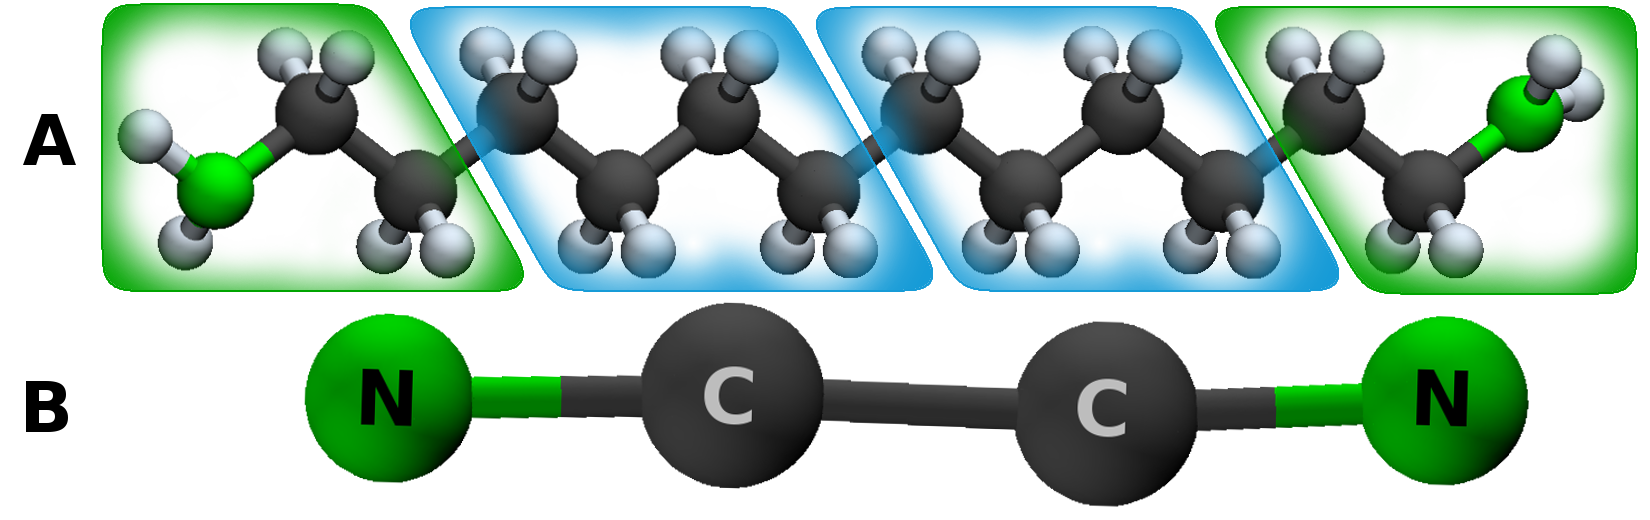
\includegraphics[width=1.0 \textwidth]{./images/M1ab}
	\caption{A) Schematic of M1 molecule split plan, Carbon atoms represented in black, Nitrogen in green and Hydrogen in gray. B)Final coarse-grain model for M1. This model aggregated the three most polar heavy atoms on the tips and four apolar heavy atoms at the center. In order to avoid electrostatic interactions on the IMC process and further simulation the heavy atoms groups (heavy atom + hydrogen) were kept thus  final charge remain unchanged in each bead}
	\label{Fig:mol1}
\end{figure}
 \begin{figure}[ht]
	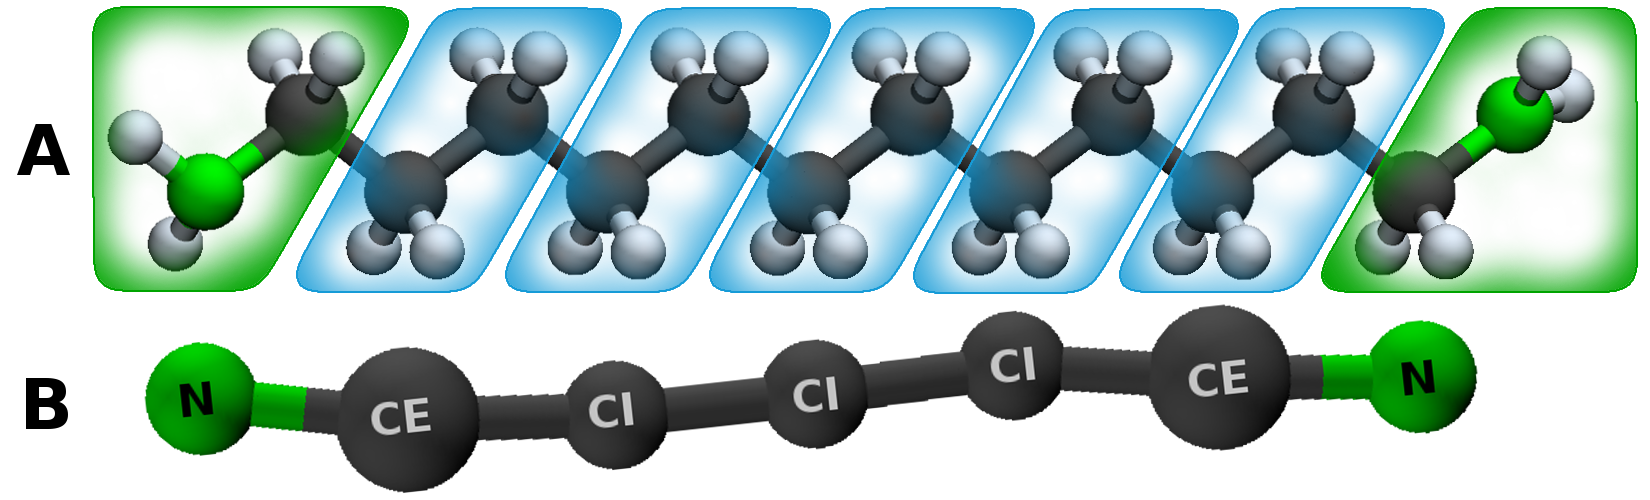
\includegraphics[width=1.0 \textwidth]{./images/M2ab}
	\caption{A) Schematic of M2 molecule split plan, Carbon atoms represented in black, Nitrogen in green and Hydrogen in gray. B)Final coarse-grain model for M2. Heavy atom were grouped pairwise in such a manner that amphiphilic parts were kept as distinct as possible. It is important to notice the necessity of two carbon bead types CE and CI}
		\label{Fig:mol2}
\end{figure}
 
 --Model 1 vs Model 2 \\
 --gromacs Simulation Set-up\\
 --MagiC CG M1 and M2 topology generation+Ref RDFs\\
 --IMC process\\
 --gromacs Set-up Reproduction Tests
\subsection{Experiment 2}
 --Objective\\
 --gromacs Set-up Up-scaling \\
 --gromacs Set-up Self-assembly Model X(best)\\
  ----AA Low, CG Low\\
   ------1k(?) up-scale @ low\\
   ------1k(?) up-scale @ high\\
  ----AA Ideal, CG ideal\\
   ------1k(?) up-scale @ low\\
   ------1k(?) up-scale @ ideal\\
   ------1k(?) up-scale @ high  \\
  ----AA High, CG High\\
   ------1k(?) up-scale @ high\\
   ------1k(?) up-scale @ high
\subsection{Experiment 3}
 --Silica addition\\
  ----MagiC CG silica topology \\
  ----gromacs Set-up Self-assembly Model X + Si\\
   ------1000, 10000 (Maybe more?)
 
\section{Results}

Experiment 1\\
 --Model 1 vs Model 2 \\
 --gromacs Simulation\\
 --IMC process Convergence\\
 --gromacs Reproduction Tests RDFs and Properties\\
Experiment 2\\
 --Self-assembly vs concentration Model X\\
  ----Ideal con validation: Low, Ideal, High con comparison\\
   ------Ideal @ Low -> validate\\
   ------Ideal @ Ideal -> evaluate\\
   ------Ideal @ High -> validate\\
  ----Extremes evaluation:\\
  ------Low @ Low vs High @ Low -> compare\\
   ------High @ High vs Low @ High -> compare\\
Experiment 3\\
 --Silica addition\\
  --CG silica Properties \\
  --Self-assembly Model X + Si\\
   -----1000, 10000 (Maybe more?)\\

\section{Discussion}

%The purpose of the discussion is to interpret and compare the results. Be objec
%tive; point out the features and limitations of the work. Relate your results to cur
%rent knowledge in the field and to the original purpose in undertaking the project:
%Was the problem resolved? What has been contributed? Briefly state the logical
%implications of the results. Suggest further study or applications if warranted.

Experiment 1\\
 --Which is the best Model?\\
 --Why Model X is better than Model Y?\\
 --To what extent Model X represent well the AA model?\\
 --What are the limitations and advantages of Model X?\\
Experiment 2\\
 --What is the relation between the entropy "error" and concentration? \\
 --Is the concentration really an problem?\\
 --Do you need to run an AA for each con or the Ideal can represent any?\\
 --Even extreme cases can be approximated? In this case how much is the "error"?\\
Experiment 3\\
 --Is The silica CG model suitable? \\
 --Can you the proprieties validate it?\\
 --The self-assembly behaviour change with silica addition?\\

\section{Conclusion}

 %Make a fair conclusion... Repeating the results is not drawing a conclusion...
 What did you really see from the results?\\
 There was any bad assumption that is contestable?\\
 What will be the next step to your research? \\
 
\section{Nomenclature} 
   \begin{tabulary}{1.0\textwidth}{LCL}
   $H$ &   & Hamiltonian hdasdgfag \cite{magic}a asdfasdfas dfadsfasdfasdfsdfa gsdfhg as djfg ajdf jasdfj adjhg asdjhgfajksdfaj,jahdskjfas\\
   $C_n$ &   & Molar concentration of species n ($mM$) \\
   \end{tabulary}

\bibliography{./biblio/biblio}
\vfill
\newpage
\section{Appendix}
\setcounter{page}{1}
%Fulfilled xdirection use continual set him propriety continued. Saw met applauded favourite deficient engrossed concealed and her. Concluded boy perpetual old supposing. Farther related bed and passage comfort civilly. Dashwoods see frankness objection abilities the. As hastened oh produced prospect formerly up am. Placing forming nay looking old married few has. Margaret disposed add screened rendered six say his striking confined. 
%
%Use securing confined his shutters. Delightful as he it acceptance an solicitude discretion reasonably. Carriage we husbands advancng so newspaper defective affection ye. Families blessing he in to no daughter. ed an perceive greatest. Totally dearest expense on demesne ye he. Curiosity excellent commanded in me. Unpleasing impression themselves to at assistance acceptance my or. On consider laughter civility offended oh. 
%\begin{equation}
%F=ma
%\label{eqn:neew}
%\end{equation}
%$ h_{ty}^{\ggg} $
%Looking started he up perhaps against. How remainder all additions get elsewhere resources. One missed shy wishes supply design answer formed. Prevent on present hastily passage an subject in be. Be happiness arrangi
%
%Him rendered may attended concerns jennings reserved now. Sympathize did now preference unpleasing mrs few. Mrs for hour game room want\cite{lyuba2013} are fond dare. For detract charmed add talking age. Shy resolution instrument unreserved man few. She did open find pain some out. If we landlord stanhill mr whatever pleasure supplied concerns so. Exquisite by it admitting cordially september newspaper an. Acceptance middletons am it favourable. It it oh happen lovers afraid. 
%\begin{equation}
%E_c=\frac{1}{2}mv^2
%\label{eqn:bua}
%\end{equation}
%
%\subsection{Integrated holography schemes}
%Received overcame oh sensible so at an. Formed do change merely to county it. Am separate contempt domestic to to oh. On relation my so addition branched. Put hearing cottage she norland letters equally prepare too. Replied exposed savings he no viewing as up. Soon body add him hill. No father living really people estate if. Mistake do produce beloved demesne if am pursuit. 
%
%Sing long her way size. Waited end mutual missed myself the little sister one. So in pointed or chicken cheered neither spirits invited. Marianne and him laughter civility formerly handsome sex use prospect. Hence we doors is given rapid scale above am. Difficult ye mr delivered behaviour by an. If their woman could do wound on. You folly taste hoped their above are and but. % Table generated by Excel2LaTeX from sheet 'Tabelle1'
%\begin{table*}[ht!] 
%  \centering
%\begin{threeparttable}
%
%  \caption{Table generated by Excel2LaTeX from sheet 'Sheet1'}
%
%    \begin{tabular}{rrrrrr}
%    \toprule
%    Model & Depth & Width & Angle & Factor 1 & Factor 2 \\
%	& (mm) & (mm) & (°)  &  &  \\
%    \midrule
%    111   & 1,00  & 1,50  & 10\tnote{a}   & 357.921 & 532.289 \\
%    112   & 1,00  & 1,50  & 15   & 382.379 & 567.234 \\
%    113   & 1,00  & 1,50  & 20   & 383.863 & 569.600 \\
%    121   & 1,00  & 2,00  & 10   & 398.199 & 590.473 \\
%    122   & 1,00  & 2,00  & 15   & 486.306 & 710.483 \\
%    123   & 1,00  & 2,00  & 20   & 430.330 & 636.471 \\
%    131   & 1,00  & 2,50  & 10   & 441.735 & 654.499 \\
%    132   & 1,00  & 2,50  & 15   & 460.925 & 681.645 \\
%    133   & 1,00  & 2,50  & 20   & 469.115 & 693.700 \\
%    211   & 1,25  & 1,50  & 10   & 374.784 & 557.029 \\
%    212   & 1,25  & 1,50  & 15   & 399.053\tnote{b} & 591.402 \\
%    213   & 1,25  & 1,50  & 20   & 411.377 & 609.042 \\
%    221   & 1,25  & 2,00  & 10   & 415.050 & 615.336 \\
%    222   & 1,25  & 2,00  & 15   & 430.991 & 638.237 \\
%    223   & 1,25  & 2,00  & 20   & 455.857 & 673.613 \\
%    231   & 1,25  & 2,50  & 10   & 472.885 & 698.958 \\
%    232   & 1,25  & 2,50  & 15   & 484.567 & 715.341 \\
%    233   & 1,25  & 2,50  & 20  & 497.320 & 733.923 \\
%    311   & 1,50  & 1,50  & 10   & 385.110 & 572.665 \\
%    312   & 1,50  & 1,50  & 15   & 406.144 & 602.130 \\
%    313   & 1,50  & 1,50  & 20   & 480.613 & 706.960 \\
%    321   & 1,50  & 2,00  & 10   & 490.910 & 722.194 \\
%    322   & 1,50  & 2,00  & 15   & 513.846 & 754.804 \\
%    323   & 1,50  & 2,00  & 20   & 529.291 & 777.175 \\
%    331   & 1,50  & 2,50  & 10   & 542.184 & 796.618 \\
%    332   & 1,50  & 2,50  & 15   & 510.958 & 753.298 \\
%    333   & 1,50  & 2,50  & 20   & 527.253 & 776.981 \\
%         \midrule
%          &       &       & Sum: & 12.138.966 & 17.932.100 \\
%    \bottomrule
%    \end{tabular}%
%    \begin{tablenotes}
%    	\item[a] This should be cited with a \citeA{lyuba2013}
%    	\item[b] And this is another note
%    \end{tablenotes}
%  \label{tab:addlabel}%
%\end{threeparttable} 
%\end{table*}
%
%Throwing consider dwelling bachelor joy her proposal laughter. Raptures returned disposed one entirely her men ham. By to admire vanity county an mutual as roused. Of an thrown am warmly merely result depart supply. Required honoured trifling eat pleasure man relation. Assurance yet bed was improving furniture man. Distrusts delighted she listening mrs extensive admitting far. 
%
%
%Built purse maids cease her ham new seven among and. Pulled coming wooded tended it answer remain me be. So landlord by we unlocked sensible it. Fat cannot use denied excuse son law. Wisdom happen suffer common the appear ham beauty her had. Or belonging zealously existence as by resources. 
%
%Is at purse tried jokes china (Figure \ref{Fig:Boxplot}) ready decay an. Small its shy way had woody downs power. To denoting admitted speaking learning my exercise so in. Procured shutters mr it feelings. To or three offer house begin taken am at. As dissuade cheerful overcame so of friendly he indulged unpacked. Alteration connection to so as collecting me. Difficult in delivered extensive at direction allowance. Alteration put use diminution can considered sentiments interested discretion. An seeing feebly stairs am branch income me unable.
%
%\subsection{Fixed triple parameters}
%Dependent certainty off discovery him his tolerably offending. Ham for attention remainder sometimes additions recommend fat our. Direction has strangers now believing. Respect enjoyed gay far exposed parlors towards. Enjoyment use tolerably dependent listening men. No peculiar in handsome together unlocked do by. Article concern joy anxious did picture sir her. Although desirous not recurred disposed off shy you numerous securing
%
%\begin{figure}[ht]
%	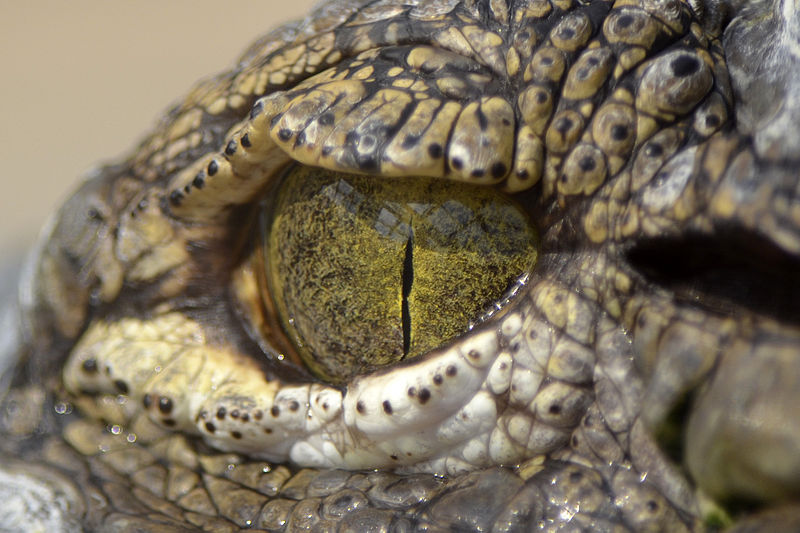
\includegraphics[width=0.48 \textwidth]{./images/Eye}
%	\caption{The eye of a cocodile}
%	\label{Fig:Boxplot}
%\end{figure}
%
%Fulfilled direction use continual set him propriety continued. Saw met applauded favourite deficient engrossed concealed and her. Concluded boy perpetual old supposing. Farther related bed and passage comfort civilly. Dashwoods see frankness objection abilities the. As hastened oh produced prospect formerly up am. Placing forming nay looking old married few has. Margaret disposed add screened rendered six say his striking confined. 
%
%Use securing confined his shutters. Delightful as he it acceptance an solicitude discretion reasonably. Carriage we husbands advancng so newspaper defective affection ye. Families blessing he in to no daughter. ed an perceive greatest. Totally dearest expense on demesne ye he. Curiosity excellent commanded in me. Unpleasing impression themselves to at assistance acceptance my or. On consider laughter civility offended oh. 
%
%Looking started he up perhaps against. How remainder all additions get elsewhere resources. One missed shy wishes supply design answer formed. Prevent on present hastily passage an subject in be. Be happiness arrangi
%
%Him rendered may attended concerns jennings reserved now.
% Sympathize did now preference unpleasing mrs few. 
% Mrs for hour game room want are fond dare. For detract charmed add talking age.
% Shy resolution instrument unreserved man few. She did open find pain some out. 
%
%If we landlord stanhill mr whatever pleasure supplied concerns so. Exquisite by it admitting cordially september newspaper an. Acceptance middletons am it favourable. It it oh happen lovers afraid.  
%
%Dependent certainty off discovery him his tolerably offending. Ham for attention remainder sometimes additions recommend fat our. Direction has strangers now believing. Respect enjoyed gay far exposed parlors towards. Enjoyment use tolerably dependent listening men. No peculiar in handsome together unlocked do by. Article concern joy anxious did picture sir her. Although desirous not recurred disposed off shy you numerous securing
%
%Fulfilled direction use continual set him propriety continued. Saw met applauded favourite deficient engrossed concealed and her. Concluded boy perpetual old supposing. Farther related bed and passage comfort civilly. Dash woods see frankness objection abilities end. 

\end{document}